% BLUEPRINTED — an investigational pamphlet
% Source for a PDF artifact; independent of the Harmonia production renderer.
% Conceptual origination: James Roy Dennis, PortusSophia(TM).
% Text prepared with PeterGate, 2026-10-08. Non-governing; no incorporation.
\documentclass[11pt]{article}
\usepackage[paperwidth=6in,paperheight=9in,top=.84in,bottom=.74in,left=.72in,right=.72in,headheight=14pt,headsep=.24in,footskip=.39in]{geometry}
\usepackage{fontspec}
\IfFileExists{/usr/share/fonts/truetype/ebgaramond/EBGaramond12-Regular.ttf}{
  \setmainfont{EBGaramond12-Regular.ttf}[Path=/usr/share/fonts/truetype/ebgaramond/, BoldFont=EBGaramond12-Bold.ttf, ItalicFont=EBGaramond12-Italic.ttf, BoldItalicFont=EBGaramond12-Italic.ttf, Ligatures=TeX]
}{\setmainfont{TeX Gyre Pagella}[Ligatures=TeX]}
\IfFileExists{/usr/share/fonts/truetype/lato/Lato-Regular.ttf}{
  \setsansfont{Lato-Regular.ttf}[Path=/usr/share/fonts/truetype/lato/, BoldFont=Lato-Bold.ttf, ItalicFont=Lato-Italic.ttf, BoldItalicFont=Lato-BoldItalic.ttf, Scale=MatchLowercase]
}{\setsansfont{TeX Gyre Heros}[Scale=MatchLowercase]}
\setmonofont{DejaVu Sans Mono}[Scale=.79]
\usepackage{tikz}
\usetikzlibrary{calc,arrows.meta,decorations.pathreplacing,backgrounds}
\usepackage{xcolor}
\definecolor{ink}{HTML}{193246}
\definecolor{deep}{HTML}{102838}
\definecolor{sea}{HTML}{427078}
\definecolor{gold}{HTML}{B48B4C}
\definecolor{cream}{HTML}{F9F6F0}
\definecolor{pale}{HTML}{ECE6D9}
\definecolor{muted}{HTML}{596976}
\definecolor{ghost}{HTML}{D7E0DD}
\usepackage[colorlinks=true,linkcolor=ink,urlcolor=sea]{hyperref}
\usepackage{fancyhdr}
\usepackage{ragged2e}
\usepackage{setspace}
\usepackage{titlesec}
\usepackage{enumitem}
\setlength{\parindent}{0pt}
\setlength{\parskip}{.58em}
\setstretch{1.095}
\AtBeginDocument{\RaggedRight\color{ink}}
\pagestyle{fancy}
\fancyhf{}
\fancyhead[L]{\sffamily\fontsize{7}{8}\selectfont\color{muted} BLUEPRINTED}
\fancyhead[R]{\sffamily\fontsize{7}{8}\selectfont\color{muted} PORTUSSOPHIA\texttrademark}
\fancyfoot[C]{\sffamily\fontsize{8}{9}\selectfont\color{gold}\thepage}
\renewcommand{\headrulewidth}{0pt}
\renewcommand{\footrulewidth}{0pt}
\titleformat{\section}{\normalfont\fontsize{18}{20}\selectfont\color{deep}}{}{0pt}{}
\titlespacing*{\section}{0pt}{.2em}{.7em}
\newcommand{\kicker}[1]{\vspace*{.10in}{\sffamily\fontsize{8.5}{10.5}\selectfont\color{gold}\MakeUppercase{#1}}\par\vspace{.12in}}
\newcommand{\sectitle}[1]{{\fontsize{20}{22}\selectfont\color{deep}#1\par}\vspace{.12in}}
\newcommand{\subhead}[1]{\par\vspace{.07in}{\sffamily\bfseries\fontsize{9.5}{11}\selectfont\color{sea}\MakeUppercase{#1}}\par\vspace{.025in}}
\newcommand{\ruleline}{\par\vspace{.13in}{\color{gold}\rule{.48in}{.9pt}}\par\vspace{.14in}}
\newcommand{\tagline}[1]{{\color{sea}\itshape\fontsize{13}{16}\selectfont #1\par}}
\newcommand{\qline}[1]{\begin{center}\begin{minipage}{.88\linewidth}\centering\color{deep}\fontsize{14}{17}\selectfont\itshape #1\end{minipage}\end{center}}
\newcommand{\notelabel}[1]{{\sffamily\fontsize{8}{9}\selectfont\color{gold}\MakeUppercase{#1}}}
\newcommand{\breakpage}{\clearpage}
\begin{document}
\thispagestyle{empty}
\pagecolor{deep}
\color{cream}

\vspace*{.65in}
{\sffamily\fontsize{9.2}{12}\selectfont\color{gold}\addfontfeatures{LetterSpace=1.7} PORTUSSOPHIA  /  CONCEPTUAL PAMPHLET\par}
\vspace{.38in}
{\fontsize{36}{36}\selectfont BLUEPRINTED\par}
\vspace{.18in}
{\fontsize{20}{23}\selectfont The Epistemic\par Aesthetics\par Inspired by\par \textit{The Last Supper}\par}
\vspace{.25in}
\begin{center}
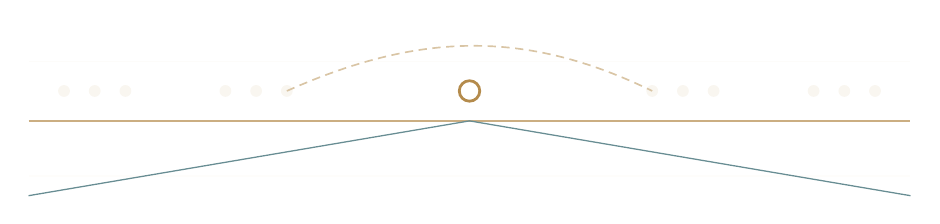
\begin{tikzpicture}[x=1cm,y=1cm]
  % A compositional study, not a reproduction of the painting.
  \draw[cream!30,line width=.45pt] (0,1.85) -- (11.2,1.85);
  \draw[gold!70,line width=.65pt] (0,1.1) -- (11.2,1.1);
  \draw[cream!25,line width=.45pt] (0,.4) -- (11.2,.4);
  \foreach \x in {.45,.84,1.23,2.50,2.89,3.28,7.92,8.31,8.70,9.97,10.36,10.75} {
    \fill[cream] (\x,1.48) circle (.075);
  }
  \draw[gold,line width=1pt] (5.60,1.48) circle (.13);
  \draw[sea!80,line width=.46pt] (0,.15) -- (5.60,1.1) -- (11.2,.15);
  \draw[gold!50,densely dashed,line width=.6pt] (3.28,1.48) to[out=24,in=154] (7.92,1.48);
\end{tikzpicture}
\end{center}
\vfill
{\fontsize{12}{16}\selectfont\color{cream!95} A necessary gap. Distinguishable figures.\par Possible relation without compelled integration.\par}
\vspace{.37in}
{\sffamily\fontsize{8.7}{12}\selectfont\color{gold} JAMES ROY DENNIS  /  PORTUSSOPHIA\texttrademark\par}
{\sffamily\fontsize{7.5}{10}\selectfont\color{cream!76} Investigational essay prepared with PeterGate  \textbullet\  8 October 2026\par}
\vspace{.14in}
\breakpage
\nopagecolor
\color{ink}
\kicker{01 / The proposition}
\sectitle{What the blank does not say}
\tagline{The space between figures is not a verdict about their relevance.}
\ruleline
Our first mistake was modest: we looked at an empty interval in a manuscript and called it spacing. The second mistake was more consequential: we began to assign the interval a job before we had examined what could happen across it.

In \textit{Integral: Epistemic Integration}, prose, accretion, distinction, and renewed prose can appear in sequence. The eye meets them one after another. Yet the sequence does not establish that one item explains the next, nor that the space between them proves irrelevance.

\vspace{.08in}
\qline{The necessary gap is not warrant for non-relevancy.}
\vspace{.04in}
The gap is a condition of distinguishability. Within or across it, distinctions \textit{may or may not} meta-engage: something at one level of examination may become consequential to another without becoming identical to it.

The interval may be empty; inquiry may seek a missing distinction or explanation there. But seeking does not establish that anything was missing, and a possible integration is not a promised one.

\vfill
{\color{sea}\fontsize{11}{14}\selectfont\itshape This pamphlet asks what visual composition can preserve that a line of symbols too easily pre-decides.\par}
\breakpage
\kicker{02 / The encounter}
\sectitle{Leonardo's arranged field}
Leonardo da Vinci's \textit{The Last Supper} shows a shared event and differentiated responses. Twelve apostles are arranged in four groups of three around Christ. Gestures move within and between the groups. Architectural perspective brings the scene toward a central point.\textsuperscript{1,2}

Those observations concern the painting's visible composition and the ordinary art-historical account of it. The following epistemic interpretation is ours, \textit{not} a claim that Leonardo devised PortusSophia's concepts.

What makes the scene instructive is not simply that it contains groups. It is that the groups remain legible without being sealed from one another. Figures face, gesture toward, recoil from, and attend across intervals. Their differences survive common participation.

A reader can explore several relations at once: the gaze of one figure, the turn of another, an interruption at the edge of a cluster, the quietness of the center, the tension between geometry and movement. These relationships do not wait for the viewer to finish reading a line.

\vspace{.08in}
\qline{Position offers orientation. Gesture invites relation. Neither establishes the whole meaning.}
\vspace{.06in}
Leonardo's painted setting is not just an ordered roster of people. It is a field of co-present distinctions. That is what makes it a fruitful inspiration for epistemic aesthetics: the work can be viewed as a composition in which space permits relations to be examined without spelling each relation out as a sentence.

\vfill
\notelabel{Boundary}  No hidden code is alleged; no theological conclusion is derived from these layout observations.
\breakpage
\kicker{03 / A study in simultaneity}
\sectitle{The field is not an arrow}
\vspace{.17in}
\begin{center}
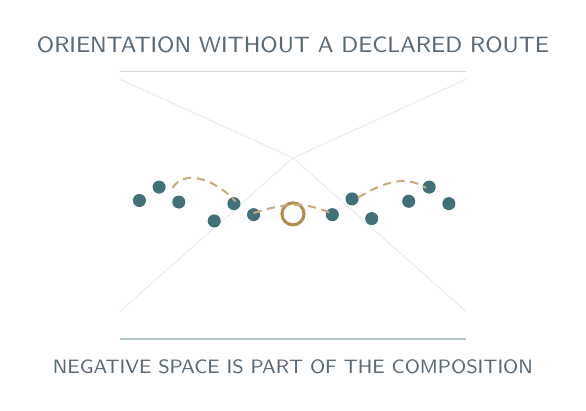
\begin{tikzpicture}[x=1cm,y=1cm]
  \draw[sea!40,line width=.6pt] (.05,.9) -- (4.45,.9);
  \draw[sea!25,line width=.45pt] (.05,4.3) -- (4.45,4.3);
  \draw[sea!13,line width=.35pt] (.05,1.25) -- (2.25,3.2) -- (4.45,1.25);
  \draw[sea!13,line width=.35pt] (.05,4.2) -- (2.25,3.2) -- (4.45,4.2);
  \foreach \x/\y in {.30/2.66,.55/2.83,.80/2.64,1.25/2.40,1.50/2.62,1.75/2.48,2.75/2.48,3.00/2.68,3.25/2.43,3.72/2.65,3.98/2.83,4.23/2.62} {
    \fill[sea] (\x,\y) circle (.083);
  }
  \draw[gold, line width=1.1pt] (2.25,2.49) circle (.14);
  % Encounters are not asserted: curved dotted lines mark possible visual traversals.
  \draw[gold!72,densely dashed,line width=.75pt] (.72,2.82) to[out=57,in=132] (1.52,2.65);
  \draw[gold!72,densely dashed,line width=.75pt] (1.75,2.50) to[out=18,in=156] (2.73,2.50);
  \draw[gold!72,densely dashed,line width=.75pt] (3.08,2.70) to[out=30,in=148] (3.94,2.82);
  \node[font=\sffamily\fontsize{8}{9}\selectfont,text=muted] at (2.25,4.64) {ORIENTATION WITHOUT A DECLARED ROUTE};
  \node[font=\sffamily\fontsize{7.5}{9}\selectfont,text=muted] at (2.25,.55) {NEGATIVE SPACE IS PART OF THE COMPOSITION};
\end{tikzpicture}
\end{center}
\vspace{.16in}
{\fontsize{10.4}{13}\selectfont\color{muted}\itshape Analytical illustration, not a reconstruction of Leonardo's figures or an assigned mapping of persons. Twelve marks, four visual groupings, and a distinct center recall the painting's compositional organization. Dashes suggest places a viewer might examine; they do not certify any relationship.\par}
\vspace{.26in}
The diagram allows several groups to coexist without requiring a single path through them. Its gaps distinguish without isolating. A viewer may notice one relation, several, or none of the proposed crossings.

An image, however, is not self-validating. What is visible must still be distinguished from what has been inferred.
\breakpage
\kicker{04 / Three different absences}
\sectitle{Absent. Missing. Forgotten.}
\subhead{Absent}
Not present at the examined location or moment. Absence is a description, not by itself a deficit. What is absent need not be supplied.
\subhead{Missing}
Not available where there is a warranted expectation of presence. To call something missing requires an account of why it belongs there. The gap alone cannot provide that account.
\subhead{Forgotten}
Previously known, encountered, or available, yet no longer carried by present attention or retrieval. What is forgotten may be recoverable; recovery is not the same as invention.
\par\vspace{.12in}\noindent
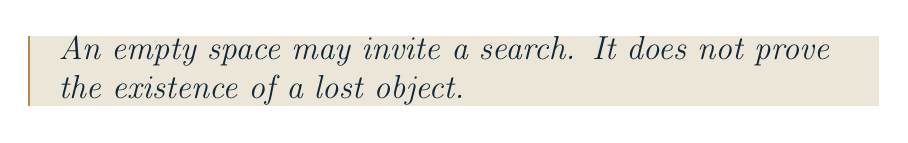
\begin{tikzpicture}
\fill[pale] (0,0) rectangle (10.8,.90);
\draw[gold,line width=1pt] (0,0) -- (0,.90);
\node[align=left,text width=10.1cm,anchor=west,font=\fontsize{12.2}{14}\selectfont\itshape,text=deep] at (.25,.45) {An empty space may invite a search. It does not prove the existence of a lost object.};
\end{tikzpicture}\par
\vspace{.12in}
These conditions may overlap in a particular case; they are not synonyms. A forgotten explanation may now be missing from an account. But an unoccupied interval may be neither missing nor forgotten.

That distinction matters for integration. If the reader is required to imagine a missing link in every gap, the presentation has already prescribed the kind of return inquiry must make. If the possibility of relation is foreclosed merely because nothing is inscribed, the presentation has made the opposite error.
\vfill
\tagline{The necessary gap permits examination without preselecting its answer.}
\breakpage
\kicker{05 / The ASCII temptation}
\sectitle{When the placeholder travels}
The manuscript's opening relation is useful precisely because it is local:
\vspace{.13in}
\begin{center}
\begin{minipage}{.83\linewidth}
\centering
{\sffamily\fontsize{9.5}{13.5}\selectfont\color{sea}
DEPTH CORRESPONDENCE\par
\vspace{.05in}
\fontsize{14}{18}\selectfont $\downarrow$\par
{\color{gold}\fontsize{13}{18}\selectfont ???}\par
\fontsize{14}{18}\selectfont $\downarrow$\par
\fontsize{9.5}{13.5}\selectfont INTEGRATION\par}
\end{minipage}
\end{center}
\vspace{.13in}
There the question marks protect an unsettled question: what, if anything, would have to be established before depth correspondence could responsibly be called integration?

Repeated elsewhere, the same marks began to function as though every interval presented the same question. A device that once kept inquiry open started narrowing the field of relevancy. It made different situations look like identical vacancies awaiting identical solutions.

\qline{The first notation did a local job. Its repetition did not inherit that job.}
\vspace{.04in}
ASCII favors succession: one line follows another; arrows suggest passage; a blank can appear to be an unfilled slot. None is inherently wrong. But the visual grammar is easy to mistake for an epistemic conclusion.

A composition may instead hold multiple distinctions visibly present at once, with no automatic hierarchy among their possible encounters. It can invite inquiry at different depths while leaving the terms distinguishable.
\breakpage
\kicker{06 / From canvas to composition}
\sectitle{What Harmonia could learn}
Harmonia need not copy Leonardo's figures or turn every piece of prose into an illustration. The opportunity is more exact: allow a rendering to carry distinctions \textit{and} the necessary space within which they might meta-engage.

\vspace{.04in}
\subhead{Prose}
Sustains argument and keeps its qualifications accountable.
\subhead{Accretion}
Holds contributions in sequence without presuming a conclusion.
\subhead{Necessary gap}
Protects distinguishability without declaring irrelevance. Engagement remains possible, not compulsory.
\subhead{Distinction}
Marks what is set apart without absorbing its neighbors.
\subhead{Return to prose}
Tests consequence without merely repeating emphasis.
\ruleline
These are compositional possibilities, not an authorized grammar. A renderer can allocate space and preserve legibility; it cannot award a relation the standing of integration because its arrangement is elegant.

\vspace{.12in}
\tagline{An image may invite passage; it cannot confer warrant.}
\breakpage
\kicker{07 / A closing bearing}
\sectitle{Blueprinted, not predetermined}
A blueprint appears to tell us where everything goes. Here it instead makes the conditions of visual inquiry inspectable without predetermining the outcome.

Leonardo's \textit{The Last Supper} presents composed plurality: a centered perspective and distinguishable figures whose gestures invite more than one route of attention. That encounter opens a question for the manuscript page.

\vspace{.08in}
\qline{Can typography and image preserve the possibility of relation without claiming that the relation is already established?}
\vspace{.05in}
The necessary gap is neither unused space nor a command to complete a pattern. It is an interval where distinctions may or may not meta-engage. The reader is invited to see; the work remains answerable for what it shows.

\ruleline
\notelabel{Provenance and standing}\par
{\fontsize{9.5}{11.5}\selectfont The distinctions on the necessary gap and possible meta-engagement originate with James Roy Dennis, Architect of PortusSophia\texttrademark. Prepared with PeterGate at his request, this is an \textbf{investigational, non-governing draft}; it does not amend \textit{Integral}, implement Harmonia, or attribute this vocabulary to Leonardo.\par}
\vspace{.09in}
\notelabel{Selected art-historical references}\par
{\fontsize{8.2}{9.5}\selectfont
1. Khan Academy / Smarthistory, \href{https://www.khanacademy.org/humanities/art-history/renaissance-reformation/high-ren-florence-rome/leonardo-da-vinci/v/leonardo-da-vinci-last-supper-1495-98}{\textit{Leonardo da Vinci, Last Supper (1495--98)}}.\par
2. \textit{Leonardo a Milano}, ``Last Supper: setting and composition,'' on the groups of three and their linked movements.\\
\href{https://www.leonardoamilano.org/english/last_supper.php}{Leonardo a Milano: The Last Supper}.\par}
\vspace{.10in}
{\sffamily\fontsize{9}{11}\selectfont\color{sea} Faith -- Fellowship -- Joy.  Here and Now!\par}
\end{document}